
\documentclass[11pt,a4paper]{article}

\usepackage[spanish,es-tabla]{babel}
\usepackage[utf8]{inputenc}
\usepackage[T1]{fontenc}
\usepackage{lmodern}
\usepackage[a4paper,margin=2.2cm]{geometry}
\usepackage{setspace}
\usepackage{graphicx}
\usepackage{float}
\usepackage{booktabs}
\usepackage{longtable}
\usepackage{amsmath}
\usepackage{array}
\usepackage{caption}
\usepackage{subcaption}
\usepackage{xcolor}
\usepackage{hyperref}
\usepackage{enumitem}
\usepackage{pdflscape}

\hypersetup{
    colorlinks=true,
    linkcolor=blue!60!black,
    urlcolor=blue!60!black,
    citecolor=blue!60!black
}

\graphicspath{{figuras/}}
\setstretch{1.03}
\setlength{\parskip}{0.35em}
\setlength{\parindent}{0pt}

\title{\textbf{Trabajo Práctico N.º 1 - Grupo 2}\\
\large Caracterización de la informalidad laboral en Argentina utilizando microdatos de la EPH, cuarto trimestre de 2024 y 2025}
\author{Taller de Programación - Universidad de Buenos Aires}
\date{ 05 de julio de 2026}

\begin{document}

\maketitle

\begin{center}
\textbf{Repositorio GitHub:} \url{https://github.com/PabloTallerProgramacion/TP1_Programacion_UBA.git}
\end{center}

\section{Introducción}

La Encuesta Permanente de Hogares (EPH), elaborada por el Instituto Nacional de Estadística y Censos (INDEC), permite estudiar las características sociodemográficas y laborales de la población argentina. En este trabajo se utilizan los microdatos individuales correspondientes al cuarto trimestre de 2024 y al cuarto trimestre de 2025 con el objetivo de caracterizar a la población ocupada y analizar la informalidad laboral desde una perspectiva descriptiva.

El grupo 2 trabaja con la categoría \textit{Upper-tier informal wage employees}, siguiendo la clasificación propuesta por Maurizio y Monsalvo (2021). Dado que la EPH no identifica directamente esta categoría como una variable observada, se construyó una aproximación empírica a partir de la categoría ocupacional, el registro previsional y el tamaño del establecimiento. En particular, se consideró como asalariado informal \textit{upper-tier} a quien cumple simultáneamente tres condiciones: ser asalariado, no contar con descuento jubilatorio y trabajar en un establecimiento de más de cinco personas.

% -------------------------------------------------
% 2. Datos y metodología
% -------------------------------------------------

\section{Datos y metodología}

La base de datos utilizada corresponde a los microdatos individuales de la EPH para el cuarto trimestre de 2024 y el cuarto trimestre de 2025. Para ambos años se seleccionaron variables de identificación, características sociodemográficas, condición de actividad, categoría ocupacional, características del empleo e ingresos.

Las variables de identificación conservadas fueron \texttt{CODUSU}, \texttt{ANO4}, \texttt{TRIMESTRE}, \texttt{NRO\_HOGAR}, \texttt{COMPONENTE} y \texttt{PONDERA}. Entre las variables de análisis se incluyeron \texttt{CH04}, \texttt{CH06}, \texttt{CH07}, \texttt{CH08}, \texttt{NIVEL\_ED}, \texttt{ESTADO}, \texttt{CAT\_OCUP}, \texttt{EMPLEO}, \texttt{SECTOR}, \texttt{PP04C}, \texttt{PP04D\_COD}, \texttt{P21} y \texttt{P47T}, junto con variables complementarias asociadas a la relación laboral.

El procesamiento se realizó en Python, utilizando principalmente las librerías \texttt{pandas}, \texttt{numpy}, \texttt{matplotlib} y \texttt{seaborn}. En primer lugar, se verificó la existencia de las variables seleccionadas en ambas bases y se armonizaron sus tipos de datos. Luego se reemplazaron por valores faltantes las observaciones con ingresos negativos en \texttt{P21} y \texttt{P47T}, por considerarse codificaciones no válidas o de no respuesta.

Posteriormente, se construyeron tres bases de trabajo. La base \texttt{respondieron} contiene las observaciones con \texttt{ESTADO} distinto de cero; la base \texttt{norespondieron} contiene los casos con \texttt{ESTADO = 0}; y la base \texttt{ocupados} conserva únicamente a quienes se encuentran ocupados, es decir, observaciones con \texttt{ESTADO = 1}.

Para hacer comparables los ingresos entre ambos períodos, los valores de \texttt{P21} y \texttt{P47T} de 2024 fueron actualizados a precios de 2025 mediante un factor de actualización de 1,315. De esta forma, las comparaciones de ingresos se realizan en pesos del cuarto trimestre de 2025.


\section{Calidad de datos y valores faltantes}

Antes de realizar el análisis descriptivo se evaluó el porcentaje de valores faltantes para las variables seleccionadas, diferenciando entre la base de personas que respondieron la pregunta de condición de actividad y la submuestra de personas ocupadas.

\begin{figure}[H]
    \centering
    
\includegraphics[width=0.95\textwidth]{figuras/Figura_Heatmap_Valores_Faltantes.png}
    \caption{Porcentaje de valores faltantes por variable. EPH 2024T4 y 2025T4.}
    \label{fig:heatmap_faltantes}
\end{figure}

Como se observa en la Figura \ref{fig:heatmap_faltantes}, las variables sociodemográficas básicas, como sexo, edad, estado civil, cobertura de salud, nivel educativo y condición de actividad, presentan cobertura completa en ambas bases. En cambio, las variables asociadas a características específicas del empleo, como \texttt{EMPLEO}, \texttt{SECTOR}, \texttt{PP04C}, \texttt{PP04D\_COD}, \texttt{PP07H}, \texttt{PP07I}, \texttt{PP07J}, \texttt{PP07K}, \texttt{PP08D1} y \texttt{PP08F1}, muestran alrededor de 55\% de valores faltantes en la base de quienes respondieron.

Este patrón no necesariamente indica un problema de calidad de los datos, sino que responde al diseño del cuestionario: estas preguntas se aplican principalmente a personas ocupadas. Al restringir la muestra a ocupados, dichos valores faltantes desaparecen. En cambio, las variables de ingresos \texttt{P21} y \texttt{P47T} conservan cerca de 20\% de valores faltantes entre ocupados, lo cual refleja la no respuesta habitual en preguntas de ingresos en encuestas de hogares.

\section{Resultados descriptivos}

La Tabla \ref{tab:resumen_ocupados} presenta una síntesis de los principales indicadores laborales y sociodemográficos para la población ocupada en 2024 y 2025. Los estadísticos descriptivos completos se presentan en el Apéndice.

\begin{table}[H]
\centering
\caption{Indicadores seleccionados de la población ocupada. EPH 2024T4 y 2025T4}
\label{tab:resumen_ocupados}
\resizebox{0.75\textwidth}{!}{
\begin{tabular}{lrr}
\toprule
\textbf{Indicador} & \textbf{2024} & \textbf{2025} \\
\midrule
Ocupados muestrales & 21.132 & 19.698 \\
Edad promedio & 41,31 & 41,86 \\
Mujeres (\%) & 45,00 & 45,49 \\
Asalariados (\%) & 72,36 & 70,78 \\
Ingreso P21 promedio ajustado & 828.157 & 917.209 \\
Ingreso P47T promedio ajustado & 940.385 & 1.040.595 \\
\bottomrule
\end{tabular}
}
\begin{flushleft}
\footnotesize Nota: los ingresos de 2024 fueron actualizados a pesos de 2025 mediante un factor de actualización de 1,315.
\end{flushleft}
\end{table}

Entre 2024 y 2025 se observa una reducción del número de ocupados muestrales incluidos en el análisis. La composición demográfica se mantiene relativamente estable: la edad promedio aumenta levemente y la proporción de mujeres ocupadas permanece cercana al 45\%. En términos laborales, se observa una ligera disminución de la proporción de asalariados. Por su parte, los ingresos promedio ajustados aumentan entre ambos años, tanto para el ingreso de la ocupación principal como para el ingreso total individual.

% -------------------------------------------------
% 5. Informalidad laboral
% -------------------------------------------------

\section{Construcción del indicador de informalidad}

La definición asignada al Grupo 2 corresponde a \textit{Upper-tier informal wage employees}. Conceptualmente, esta categoría refiere a trabajadores asalariados informales ubicados en segmentos relativamente superiores dentro del empleo informal. Dado que la EPH no contiene una variable que identifique directamente esta categoría, se construyó una aproximación empírica basada en tres criterios observables.

En primer lugar, se restringió la identificación a trabajadores asalariados, utilizando la variable \texttt{CAT\_OCUP}. En segundo lugar, se consideró como informal a quienes no registran descuento jubilatorio, utilizando la variable \texttt{PP07H}. Finalmente, para aproximar el componente \textit{upper-tier}, se incorporó información del tamaño del establecimiento mediante la variable \texttt{PP04C}, clasificando como \textit{upper-tier} a los asalariados informales que trabajan en establecimientos de más de cinco personas.

Formalmente, el indicador se define como:

\[
UpperTierInformal_i =
\begin{cases}
1 & \text{si } CAT\_OCUP_i = 3,\; PP07H_i = 2,\; PP04C_i > 5 \\
0 & \text{en otro caso}
\end{cases}
\]

Esta clasificación debe interpretarse como una aproximación descriptiva a la categoría asignada, no como una reproducción exacta de la metodología de Maurizio y Monsalvo (2021).

\input{tabla_informalidad.tex}


\section{Distribución de ingresos y correlaciones}

La Figura \ref{fig:ingresos2024} muestra la distribución de los ingresos laborales para trabajadores asalariados formales y \textit{upper-tier informal wage employees} en 2024. En los histogramas y las densidades Kernel se observa que la distribución de los asalariados formales está desplazada hacia mayores niveles de ingreso, mientras que la distribución de los asalariados informales \textit{upper-tier} se concentra en tramos de ingreso más bajos. Este resultado es consistente con una segmentación persistente del mercado laboral.

\begin{figure}[H]
    \centering
    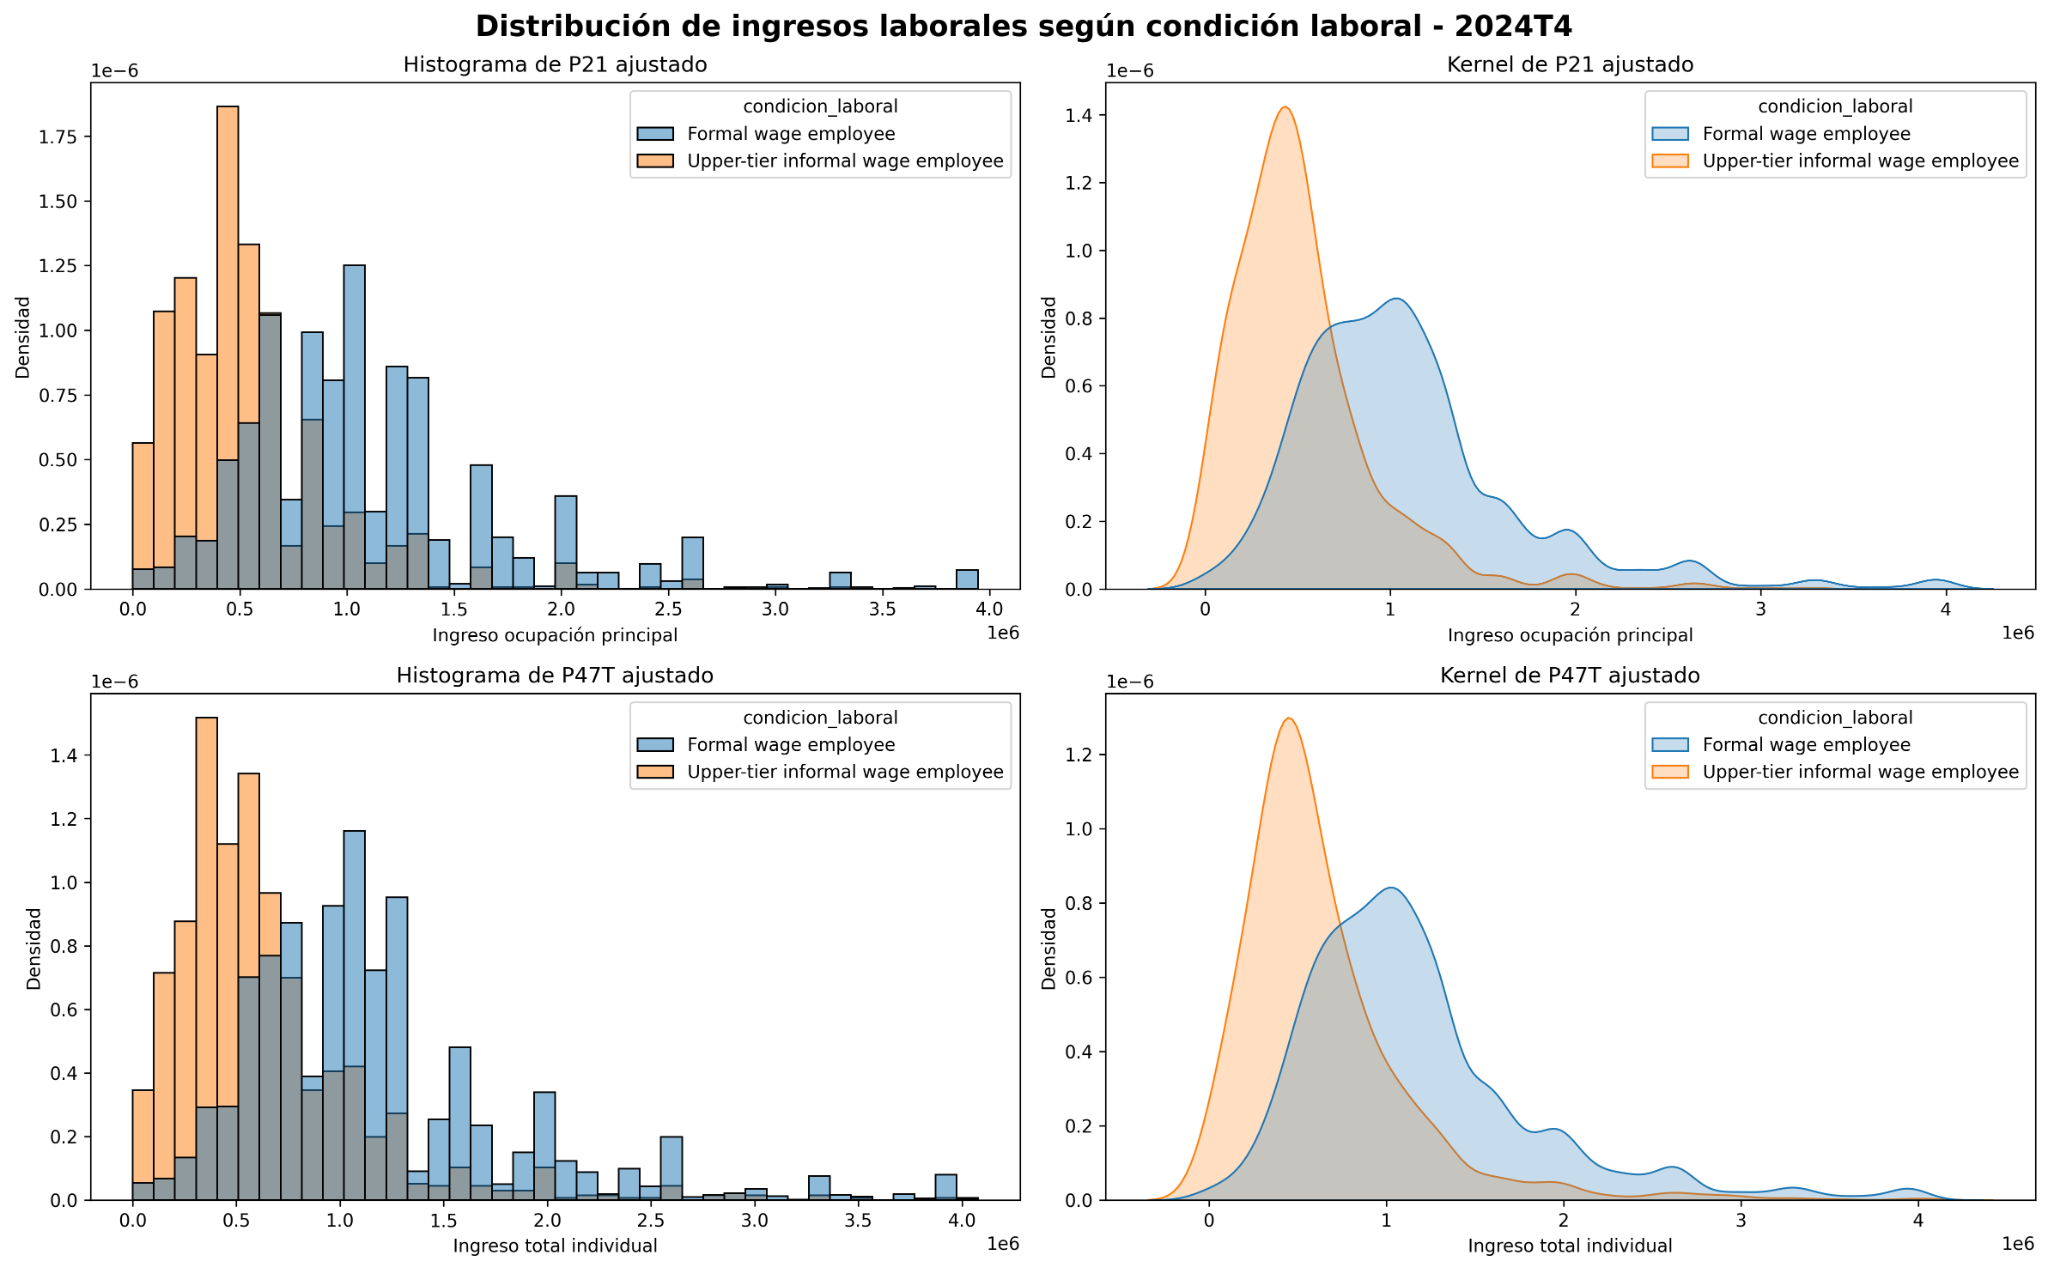
\includegraphics[width=\textwidth]{Figura_Distribucion_Ingresos_2024.png}
    \caption{Distribución de ingresos laborales según condición laboral. EPH 2024T4.}
    \label{fig:ingresos2024}
\end{figure}

Como complemento, se estimaron matrices de correlación para 2024 y 2025 (Figuras \ref{fig:corr2024} y \ref{fig:corr2025} del Apéndice). En ambos años se observa una correlación elevada entre el ingreso de la ocupación principal y el ingreso total individual. Además, el nivel educativo presenta una asociación positiva con los ingresos, mientras que el sector y la cobertura de salud exhiben asociaciones negativas con los ingresos ajustados. La variable \texttt{ESTADO} no presenta correlaciones relevantes dentro de la base de ocupados porque, por construcción, todos los individuos incluidos tienen \texttt{ESTADO = 1}.


\section{Conclusiones}

El trabajo permitió construir una primera caracterización descriptiva de la población ocupada en Argentina utilizando microdatos de la EPH para el cuarto trimestre de 2024 y 2025. El procesamiento realizado incluyó la selección y armonización de variables, la limpieza de valores atípicos, la creación de subbases de análisis y el ajuste de ingresos de 2024 a precios de 2025.

Los resultados muestran una composición demográfica relativamente estable entre ambos años, junto con un aumento de los ingresos promedio ajustados. Las matrices de correlación evidencian una fuerte asociación entre el ingreso de la ocupación principal y el ingreso total individual, así como una relación positiva entre nivel educativo e ingresos laborales.

Respecto de la informalidad, se construyó una aproximación empírica a la categoría \textit{Upper-tier informal wage employees}, asignada al Grupo 2. Esta clasificación combina información sobre categoría ocupacional, descuento jubilatorio y tamaño del establecimiento. Los resultados deben interpretarse con cautela, dado que la EPH no identifica directamente esta categoría, pero permiten realizar una aproximación descriptiva consistente con las variables disponibles.

% -------------------------------------------------
% 9. Uso de herramientas de IA
% -------------------------------------------------

\section{Uso de herramientas de Inteligencia Artificial}

Durante el desarrollo del trabajo se utilizó ChatGPT como apoyo principal para organizar y ajustar el código en Python previamente definido, verificar errores, mejorar la construcción de las tablas resultantes y orientar el guardado de archivos en Google Drive. Asimismo, se utilizó Gemini como apoyo complementario para mejorar la redacción final del informe.

No obstante, las decisiones metodológicas, la validación de los resultados y la interpretación económica fueron realizadas por el grupo, contrastando el código y los resultados obtenidos con la consigna del trabajo práctico, la documentación oficial de la EPH y la literatura utilizada como referencia.

\clearpage
\appendix

\section{Tablas complementarias}

\input{tabla_descriptiva.tex}

\input{tabla_faltantes.tex}

\section{Matrices de correlación}

\begin{figure}[H]
    \centering
    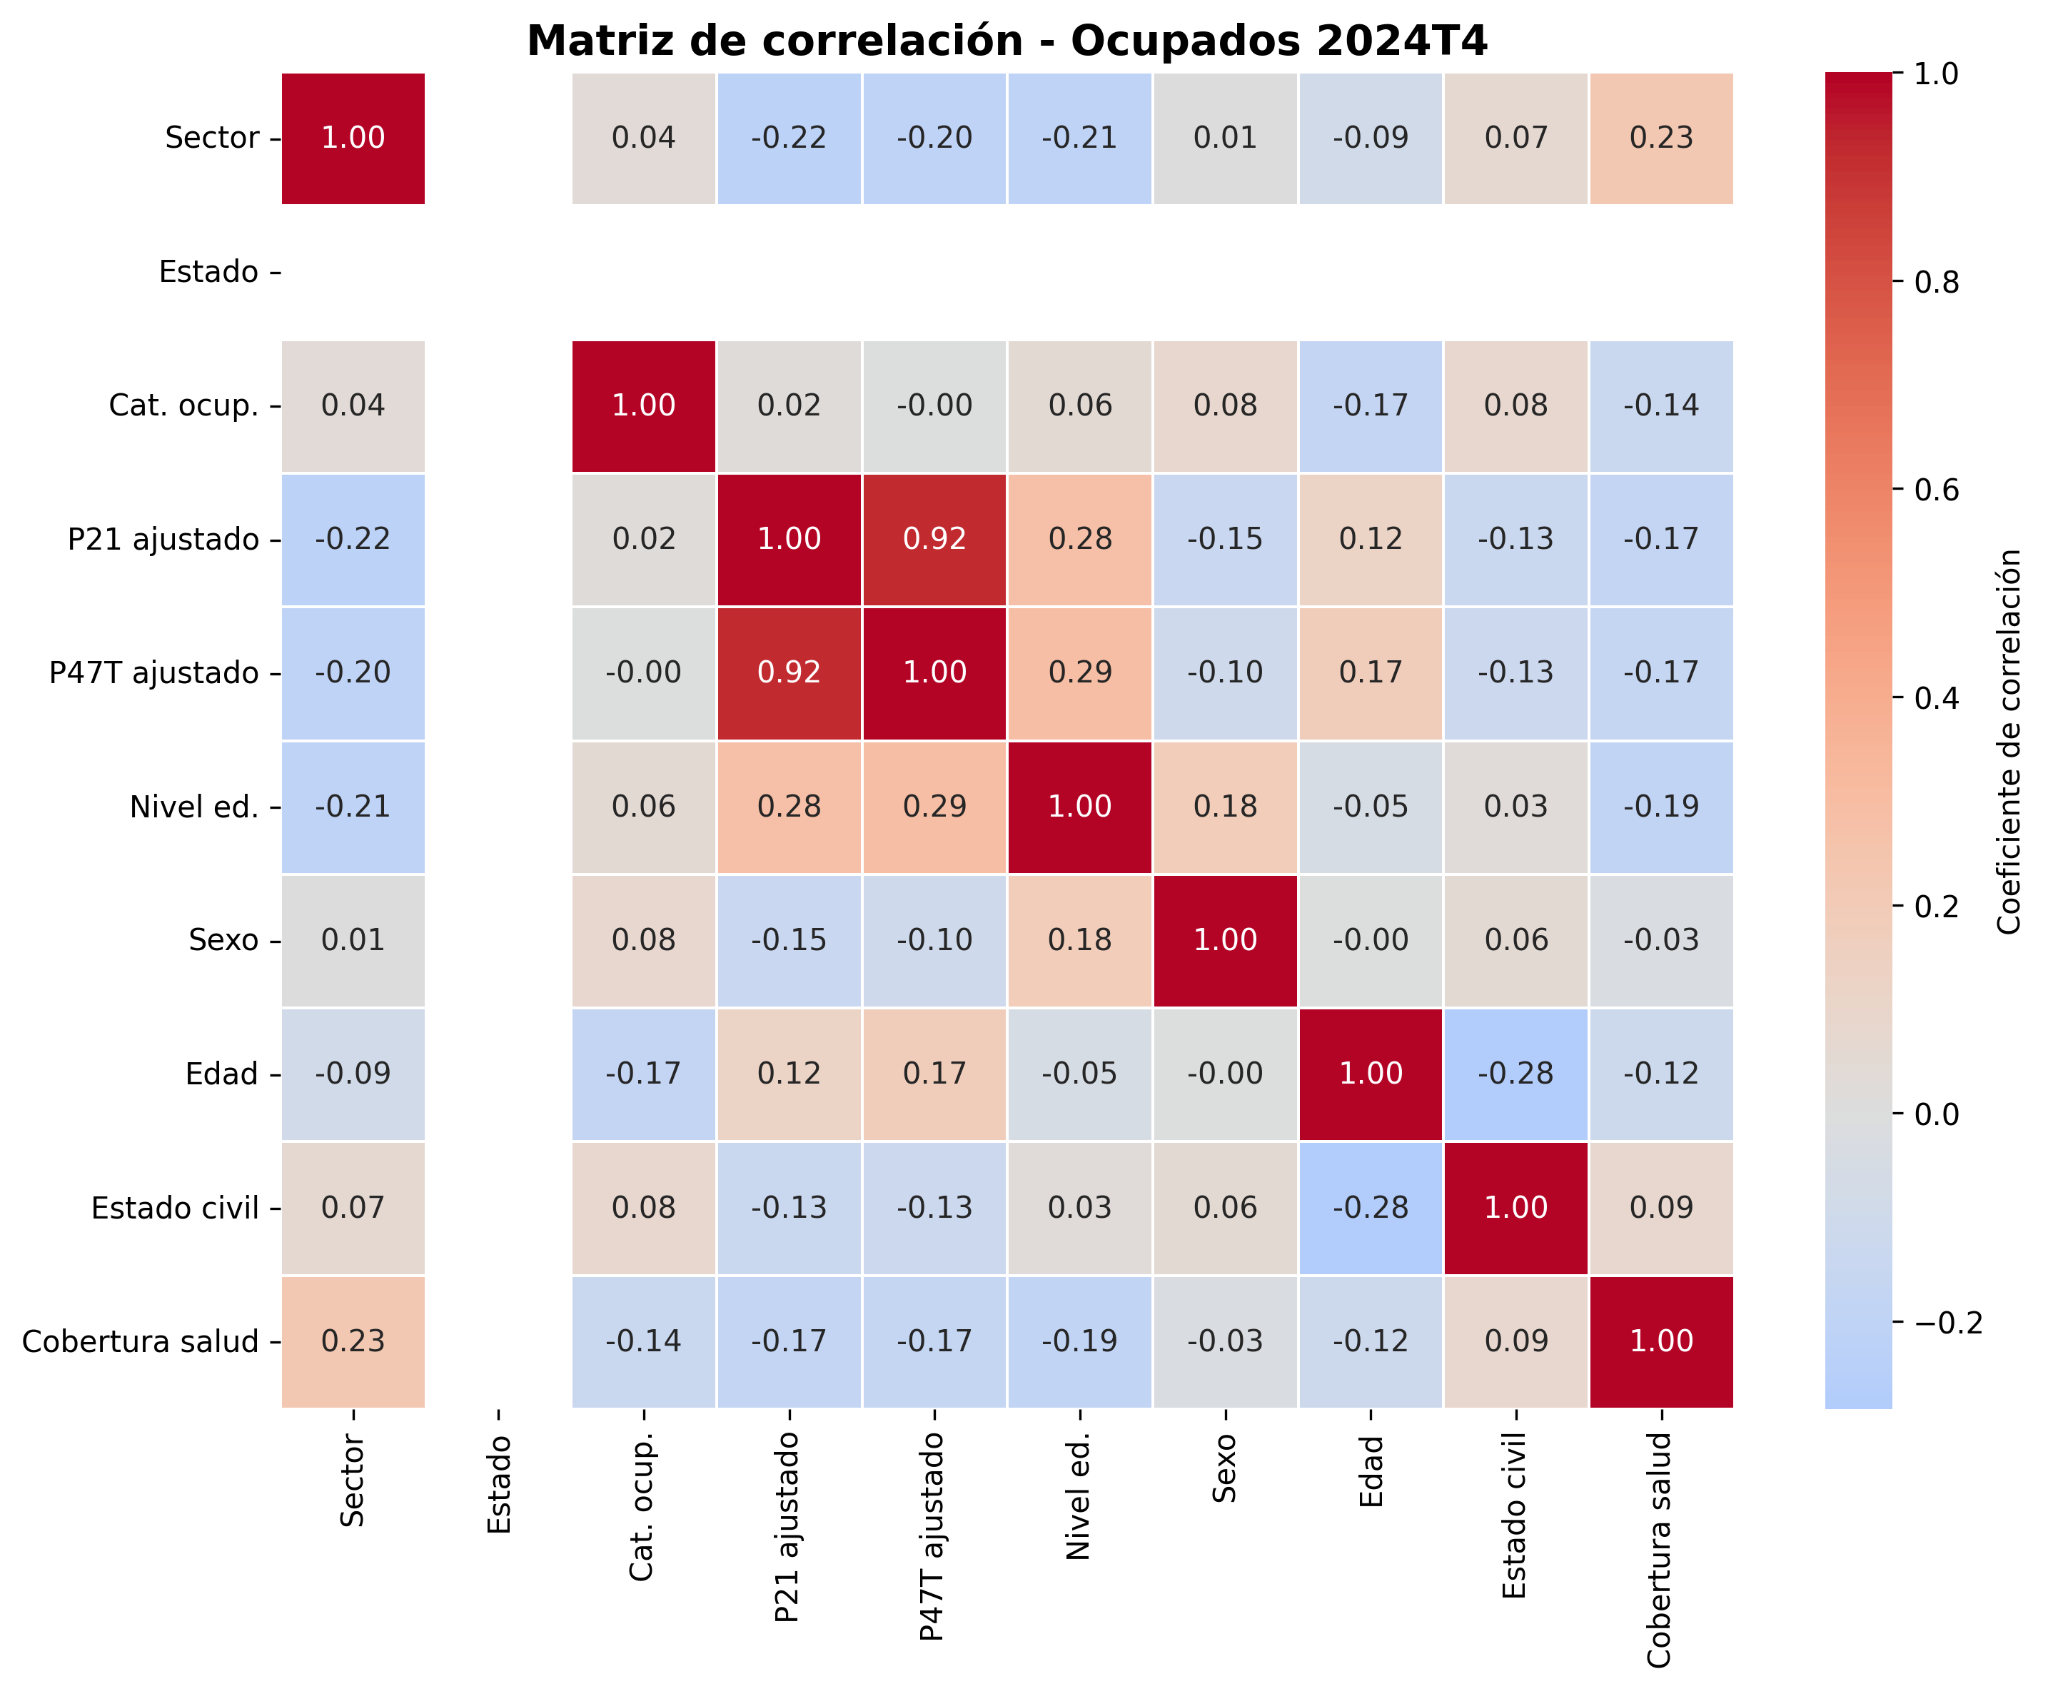
\includegraphics[width=0.88\textwidth]{Figura_Matriz_Correlacion_2024.png}
    \caption{Matriz de correlación. Población ocupada, EPH 2024T4.}
    \label{fig:corr2024}
\end{figure}

\begin{figure}[H]
    \centering
    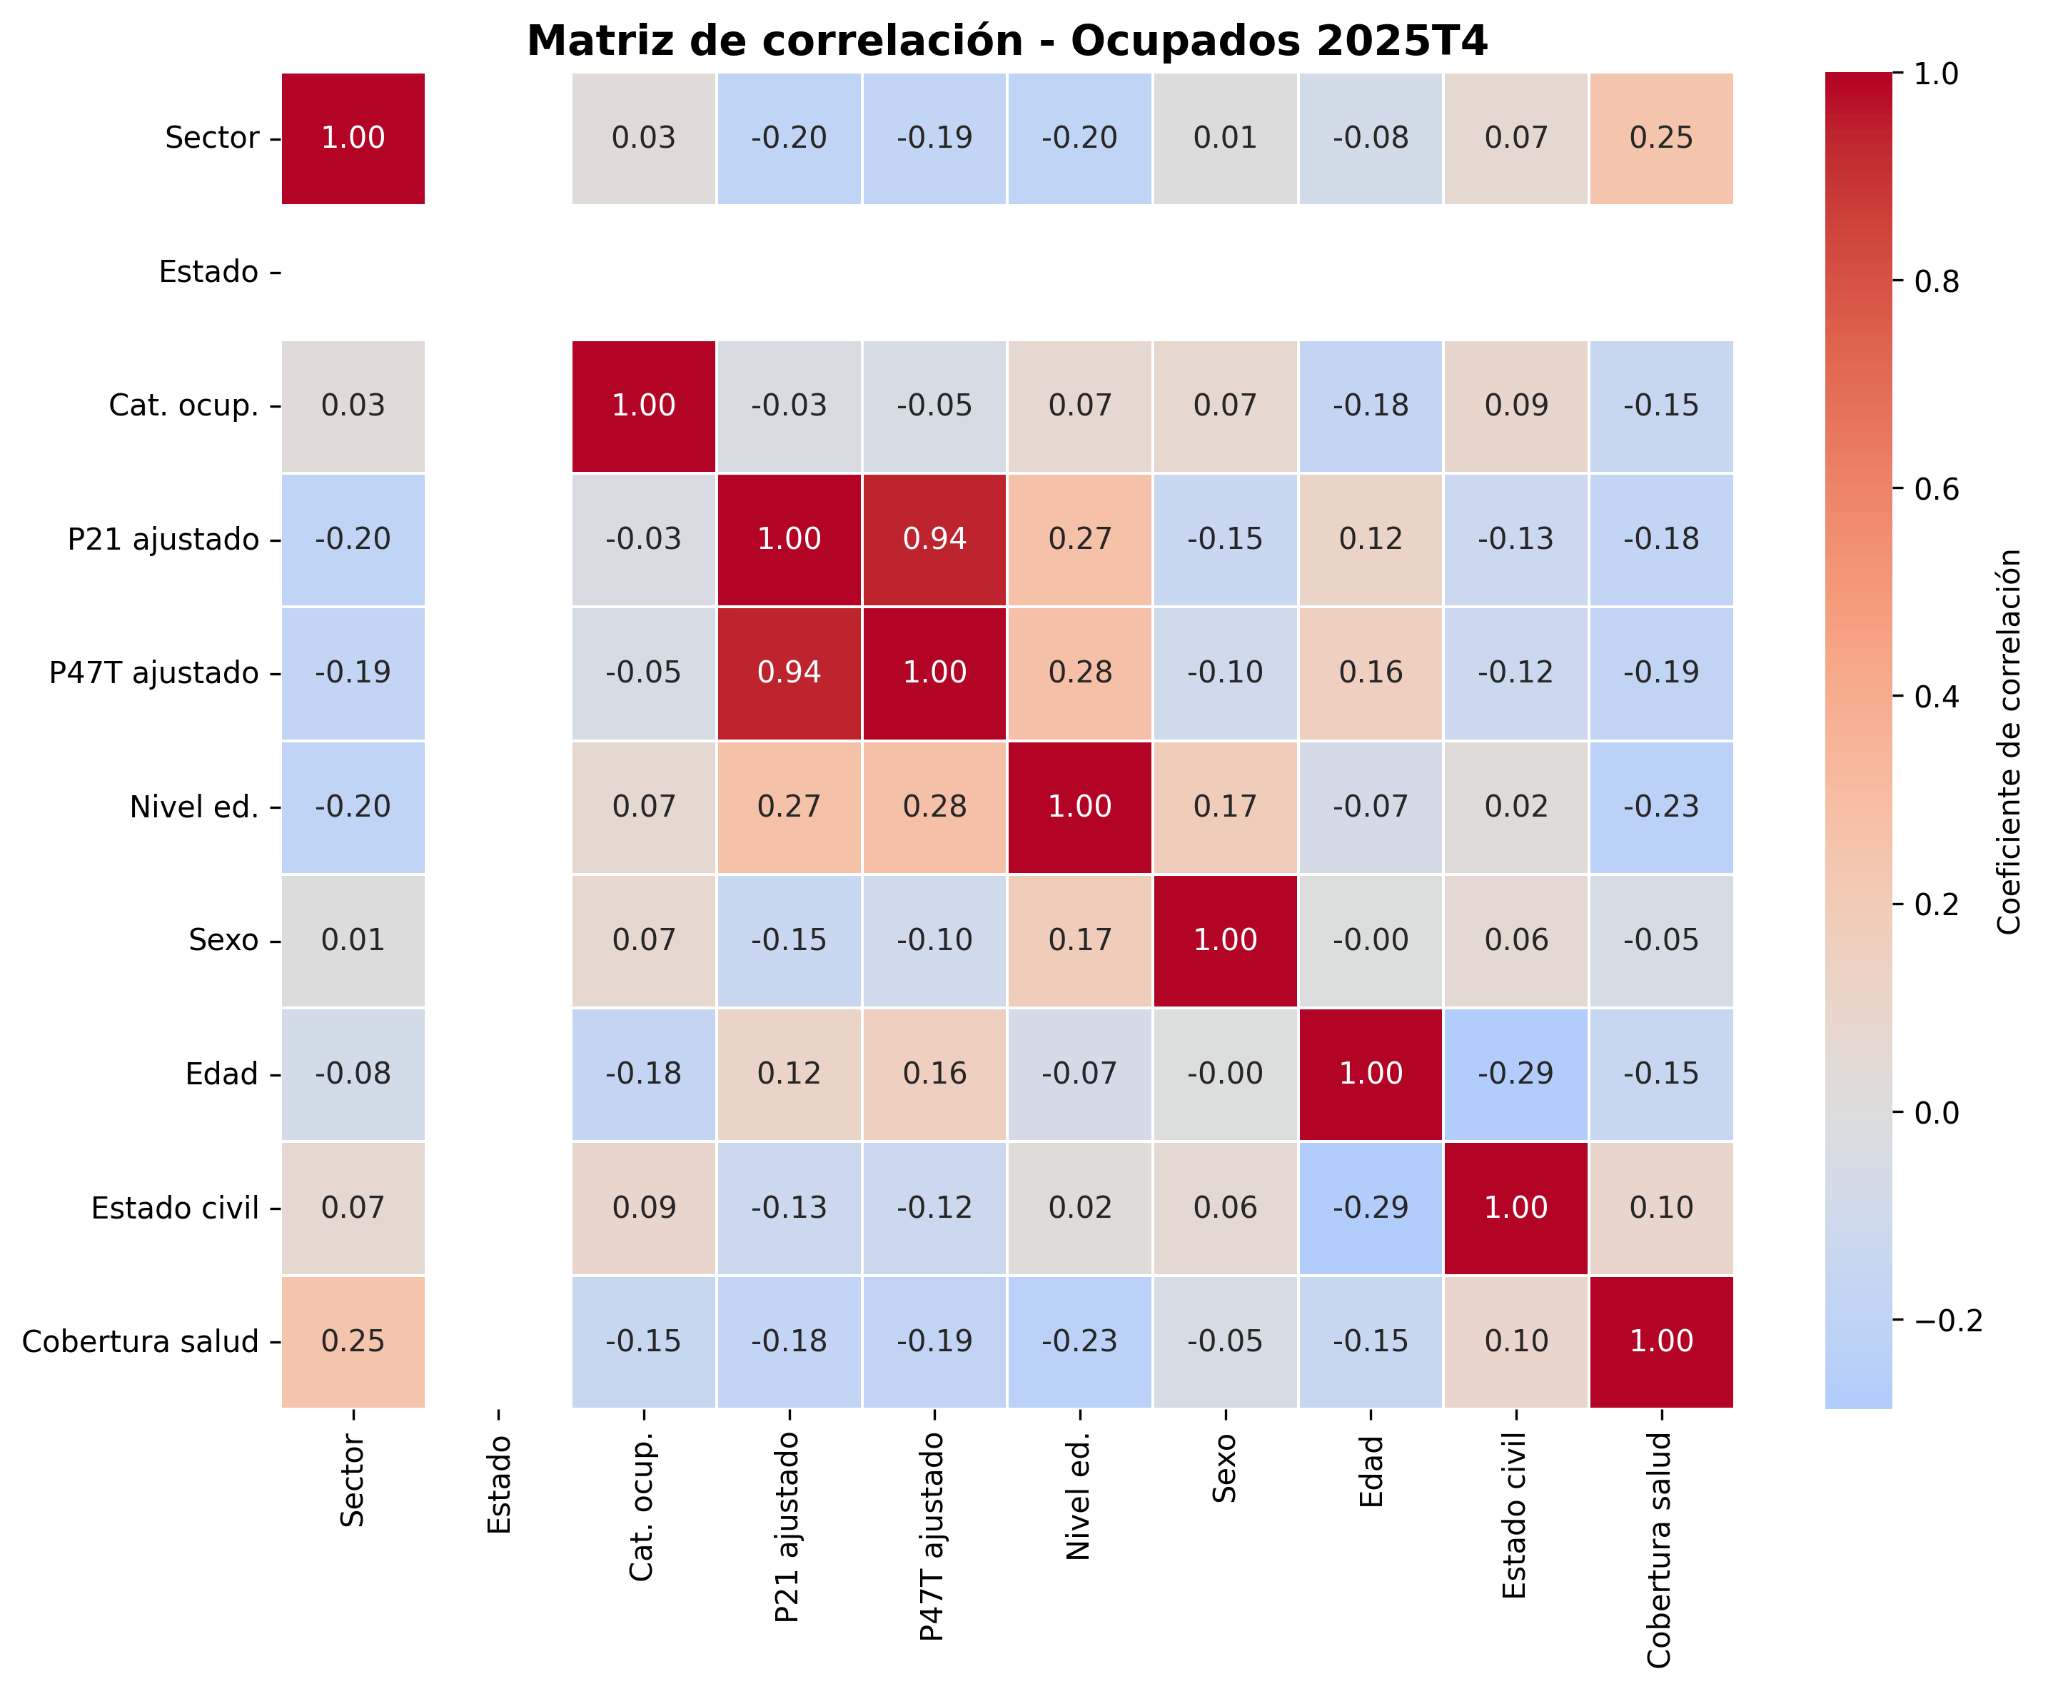
\includegraphics[width=0.88\textwidth]{Figura_Matriz_Correlacion_2025.png}
    \caption{Matriz de correlación. Población ocupada, EPH 2025T4.}
    \label{fig:corr2025}
\end{figure}

\section{Prompts principales utilizados}

\begin{enumerate}[leftmargin=*]
    \item \textit{``Realiza un análisis del código que te he entregado buscando fallas y posibles mejoras de acuerdo a la consigna específica, no alusiones ni aumentes nada que no sea requerido  ''}
    \item \textit{``detalla paso a paso y con explicaciones la mejora del código en la celda 10''}
    \item \textit{``Entregame el código necesario para guardar los archivos .xlsx que generó el códgio dentro de una carpeta drive''}
    \item \textit{``Realiza un check list y validación final del proceso del código, verifica si cumple con todo lo requerido''}

\end{enumerate}

\section{Referencias}

\begin{thebibliography}{9}

\bibitem{maurizio2021}
Maurizio, R. y Monsalvo, A. P. (2021).
\textit{Informality, labour transitions, and the livelihoods of workers in Latin America}.
WIDER Working Paper No. 2021/19. UNU-WIDER.

\bibitem{indec}
INDEC.
\textit{Encuesta Permanente de Hogares (EPH): microdatos individuales y diseño de registros}.
Instituto Nacional de Estadística y Censos, Argentina.

\bibitem{schwabish2014}
Schwabish, J. A. (2014).
An economist's guide to visualizing data.
\textit{Journal of Economic Perspectives}, 28(1), 209--234.

\end{thebibliography}

\end{document}
